\section{Method}
\label{sec:method}

Euler wave drag of each nose $\rightarrow$ vehicle drag build-up $\rightarrow$ ascent trajectory
$\rightarrow$ apogee and stability (implementation: Appendix~\ref{app:scripts}).

\subsection{Nose wave drag: axisymmetric Euler solver}
\label{sec:euler}

Above Mach 1 the nose pressure drag is set by the inviscid outer flow, so the axisymmetric Euler
equations are solved for each nose followed by a $5R$ cylinder; skin friction is added in the flight
model. In finite-volume form, per radian of azimuth,
\begin{equation}
\frac{\partial (\boldsymbol U V)}{\partial t} + \sum_{\rm faces} \boldsymbol F\cdot\boldsymbol n\, \ell\, r_f
= \begin{pmatrix} 0 & 0 & p\,A & 0 \end{pmatrix}^{\!\top},
\qquad V = A\, r_c ,
\label{eq:euler}
\end{equation}
with $\boldsymbol U = (\rho,\rho u,\rho v,E)$, $\boldsymbol F$ the flux through a face of normal
$\boldsymbol n$, length $\ell$ and mid-radius $r_f$, and $V$ the volume per radian of a cell of area $A$
and centroid radius $r_c$. Scheme: HLLC fluxes, MUSCL (minmod) reconstruction, SSP-RK2 with local time
stepping at CFL 0.85, on a $160\times80$ body-fitted grid with characteristic far field, slip wall and
symmetry axis. The wave drag is
\begin{equation}
C_{D,\rm w} = \frac{1}{q_\infty \pi R^2}\int_{\rm nose} (p-p_\infty)\,(-n_x)\, 2\pi r\,\mathrm ds .
\label{eq:cdw}
\end{equation}
A run is converged when $C_{D,\rm w}$ changes by less than $2\times10^{-5}$ over 250 iterations. Mach
numbers are run from 1.6 down to 1.1, each from the previous solution; the $M=1.1$ runs stopped at 6000
iterations (1--2\,\% uncertainty). The trade study interpolates $C_{D,\rm w}(L/D)^2$ between $L/D = 3$, 4
and 5; all shapes were also run directly at $L/D = 4.5$ ($M = 1.6$, 1.4, 1.2), and these direct values
are used at $L/D = 4.5$.

\textbf{Validation.} Against the exact Taylor--Maccoll cone solution the largest error is 0.46\,\%
(four cone angles, $M = 1.1$--2; Figure~\ref{fig:validation}a). On three grids the observed order at
$M=1.4$ is $p = 2.0$ and the GCI of the production grid 0.5\,\% (1.1\,\% at $M = 1.2$,
Figure~\ref{fig:validation}b), well below the 3--46\,\% by which the other shapes exceed Von K\'arm\'an.

\begin{figure}[H]
\centering
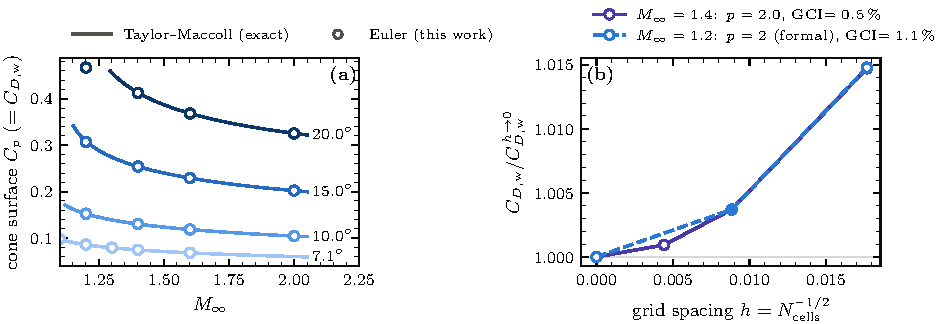
\includegraphics[width=\textwidth]{fig_validation}
\caption{(a) Cone surface pressure from the Euler solver (markers) against the exact
Taylor--Maccoll solution (lines). (b) Grid convergence of the nose wave drag, normalised by the
Richardson-extrapolated value (open: computed grids; filled: production grid).}
\label{fig:validation}
\end{figure}

\subsection{Transonic range}
\label{sec:transonic}

Below $M=1.1$ the Euler runs converge too slowly. The nose wave drag is modelled as a smooth cubic rise
from zero at $M=0.8$ to the $M=1.1$ value at $M=1.0$; its onset and amplitude are varied in the robustness
study (Section~\ref{sec:robust}), and the Fluent runs of Section~\ref{sec:next} replace it.

\subsection{Flight model}
\label{sec:flight}

A point-mass trajectory from the \SI{12}{m} rail ($84^\circ$) to apogee:
\begin{equation}
m\frac{\mathrm dV_\infty}{\mathrm dt} = F_{\rm th} - \tfrac12\rho V_\infty^2 A_b C_D - m g\sin\gamma_f ,
\qquad
V_\infty\frac{\mathrm d\gamma_f}{\mathrm dt} = -g\cos\gamma_f ,
\label{eq:eom}
\end{equation}
with linear mass decrease and the ISA, and the drag build-up
\begin{equation}
C_D = k\left(C_{D,f} + C_{D,\rm fins} + C_{D,\rm base} + C_{D,e}\right) + C_{D,\rm w}(M)
\label{eq:buildup}
\end{equation}
(Schlichting friction with compressibility and roughness, Ackeret fin drag, OpenRocket base drag, ERT-Sim
excrescences). A longer nose also adds wetted area and shell mass. $k$ is set so that the baseline nose
(Von K\'arm\'an, \SI{720}{mm}) reaches \SI{9.0}{km}; the resulting $M_{\max}=1.47$ matches the LVO's
Mach 1.4 without further tuning.

\subsection{Stability, mass and payload}

Barrowman: nose $C_{N\alpha}=2$ at $x_{cp}=L-V/A_b$, fins $C_{N\alpha,f}=7.4$; static margin
$(x_{cp} - x_{cg})/D$ with positions from the aft end and the CG shift of the shell mass included. Shell
mass $=$ wetted area $\times$ \SI{0.98}{kg/m^2}; the 3U fit is the curved length with $r\geq\SI{77}{mm}$.
